\chapter{claws}
\label{sec:claws}
\lhead[tempest 2000]{}
\lstset{style=68KStyle}

In Tempest 2000, for no good reason, the 'classic' tempest claws use trios of bytes to give
co-ordinates in 3D space. I say 'for no good reason' because the claw is still flat, so the
Z co-ordinate is always a \icode{1}. We define our claws using a list of \icode{X,Y,Z} 
co-ordinates, and each co-ordinate is paired with a list of points that it connects to. It
is this list of connecting points that allows us to draw lines:
\begin{lstlisting}
claw3:  dc.b 4,5,1                 ; Co-ordinate 1
        dc.b 2,8,0                 ; Draw line to co-ords 2 and 8.
        dc.b 4,11,1                ; Co-ordinate 2
        dc.b 3,0                   ; Draw line to co-ord 3.
        dc.b 11,12,1               ; Co-ordinate 3
        dc.b 4,0                   ; Draw line to co-ord 4.
        dc.b 15,8,1                ; Co-ordinate 4
        dc.b 5,0                   ; Draw line to co-ord 5.
        dc.b 12,4,1                ; Co-ordinate 5
        dc.b 6,0                   ; Draw line to co-ord 6.
        dc.b 17,8,1                ; Co-ordinate 6
        dc.b 7,0                   ; Draw line to co-ord 7.
        dc.b 11,15,1               ; Co-ordinate 7
        dc.b 8,0                   ; Draw line to co-ord 8.
        dc.b 2,12,1                ; Co-ordinate 8
        dc.b 0,0                   ; Don't draw a line.
\end{lstlisting}

This is what it looks like when we consume the first co-ordinate and its paired points:
\begin{lstlisting}
claw3:  dc.b 4,5,1                 ; Co-ordinate 1
        dc.b 2,8,0                 ; Draw line to co-ords 2 and 8.
\end{lstlisting}

This is telling us to connect our first trio \icode{4,5,1} to co-ordinates
'2' (\icode{4,11,1})..
\begin{figure}[H]
    \centering
    \begin{adjustbox}{width=7cm,center}
      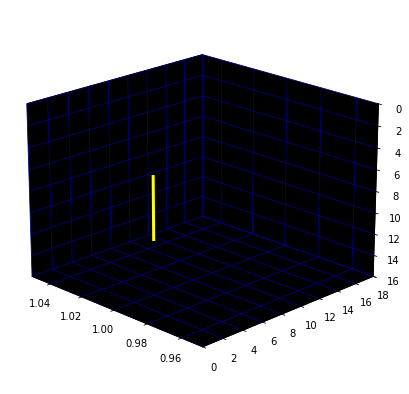
\includegraphics[width=12cm]{src/claws/build_claw_1_0.png}%
    \end{adjustbox}
  \caption*{Draw a line from \icode{(4,5,1)} to \icode{(4,11,1)}.}
\end{figure}
.. and '8' (\icode{2,12,1}).
\begin{figure}[H]
    \centering
    \begin{adjustbox}{width=7cm,center}
      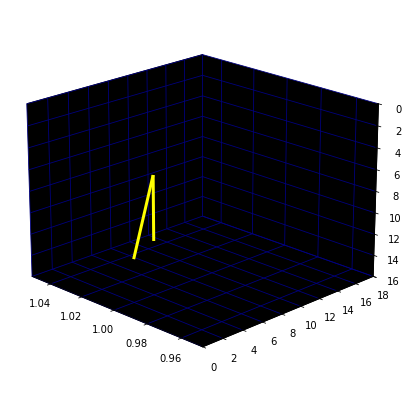
\includegraphics[width=12cm]{src/claws/build_claw_1_1.png}%
    \end{adjustbox}
  \caption*{Draw a line from \icode{(4,5,1)} to \icode{(2,12,1)}.}
\end{figure}


With this as our method, we can start building up our complete image, adding each point in
our array to the previous result to define a new line to draw.

\begin{minipage}[c]{0.48\linewidth}
\begin{figure}[H]
    \centering
    \begin{adjustbox}{width=5.5cm,center}
      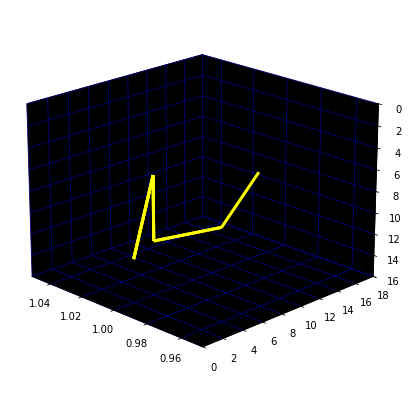
\includegraphics[width=12cm]{src/claws/build_claw_3_0.png}%
    \end{adjustbox}
\end{figure}
\end{minipage}
\begin{minipage}[c]{0.48\linewidth}
\begin{lstlisting}[basicstyle=\scriptsize\ttfamily]
dc.b 4,11,1   ; Co-ordinate 2
dc.b 3,0      ; Draw line to co-ord 3.
dc.b 11,12,1  ; Co-ordinate 3
\end{lstlisting}
\vspace*{\fill}
\end{minipage}

\begin{minipage}[c]{0.48\linewidth}
\begin{figure}[H]
    \centering
    \begin{adjustbox}{width=5.5cm,center}
      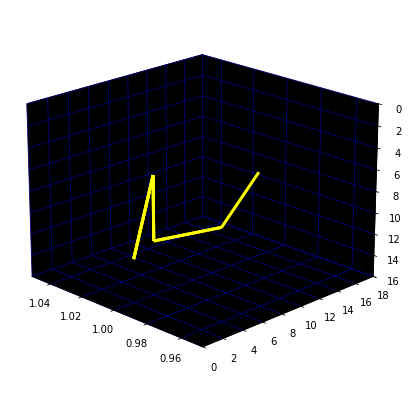
\includegraphics[width=12cm]{src/claws/build_claw_3_0.png}%
    \end{adjustbox}
\end{figure}
\end{minipage}
\begin{minipage}[c]{0.48\linewidth}
\begin{lstlisting}[basicstyle=\scriptsize\ttfamily]
dc.b 11,12,1 ; Co-ordinate 3
dc.b 4,0     ; Draw line to co-ord 4.
dc.b 15,8,1  ; Co-ordinate 4
\end{lstlisting}
\vspace*{\fill}
\end{minipage}

\begin{minipage}[c]{0.48\linewidth}
\begin{figure}[H]
    \centering
    \begin{adjustbox}{width=5.5cm,center}
      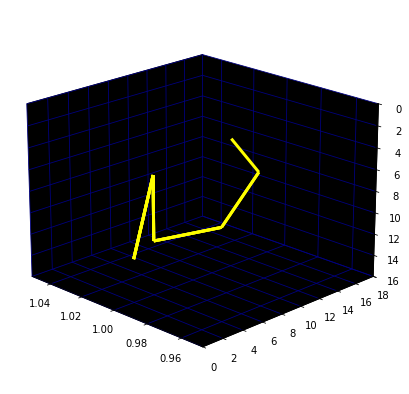
\includegraphics[width=12cm]{src/claws/build_claw_4_0.png}%
    \end{adjustbox}
\end{figure}
\end{minipage}
\begin{minipage}[c]{0.48\linewidth}
\begin{lstlisting}[basicstyle=\scriptsize\ttfamily]
dc.b 15,8,1  ; Co-ordinate 4
dc.b 5,0     ; Draw line to co-ord 5.
dc.b 12,4,1  ; Co-ordinate 5
\end{lstlisting}
\vspace*{\fill}
\end{minipage}

\begin{minipage}[c]{0.48\linewidth}
\begin{figure}[H]
    \centering
    \begin{adjustbox}{width=5.5cm,center}
      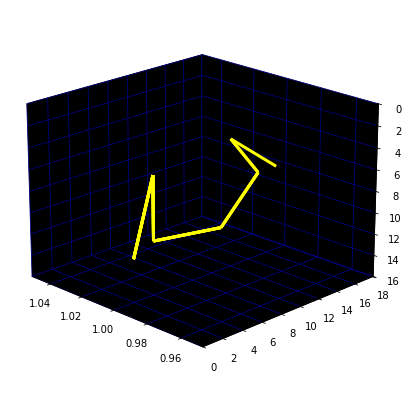
\includegraphics[width=12cm]{src/claws/build_claw_5_0.png}%
    \end{adjustbox}
\end{figure}
\end{minipage}
\begin{minipage}[c]{0.48\linewidth}
\begin{lstlisting}[basicstyle=\scriptsize\ttfamily]
dc.b 12,4,1  ; Co-ordinate 5
dc.b 6,0     ; Draw line to co-ord 6.
dc.b 17,8,1  ; Co-ordinate 6
\end{lstlisting}
\vspace*{\fill}
\end{minipage}

\begin{minipage}[c]{0.48\linewidth}
\begin{figure}[H]
    \centering
    \begin{adjustbox}{width=5.5cm,center}
      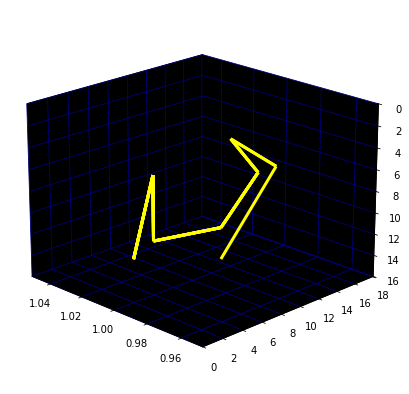
\includegraphics[width=12cm]{src/claws/build_claw_6_0.png}%
    \end{adjustbox}
\end{figure}
\end{minipage}
\begin{minipage}[c]{0.48\linewidth}
\begin{lstlisting}[basicstyle=\scriptsize\ttfamily]
dc.b 17,8,1   ; Co-ordinate 6
dc.b 7,0      ; Draw line to co-ord 7.
dc.b 11,15,1  ; Co-ordinate 7
\end{lstlisting}
\vspace*{\fill}
\end{minipage}

\begin{minipage}[c]{0.48\linewidth}
\begin{figure}[H]
    \centering
    \begin{adjustbox}{width=5.5cm,center}
      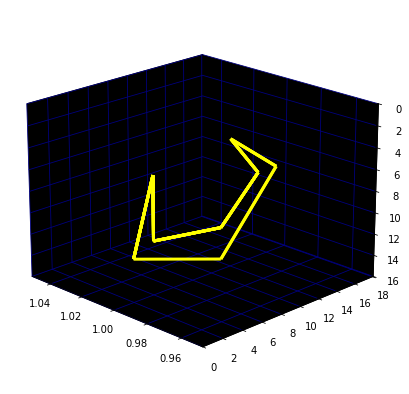
\includegraphics[width=12cm]{src/claws/build_claw_7_0.png}%
    \end{adjustbox}
\end{figure}
\end{minipage}
\begin{minipage}[c]{0.48\linewidth}
\begin{lstlisting}[basicstyle=\scriptsize\ttfamily]
dc.b 11,15,1 ; Co-ordinate 7
dc.b 8,0     ; Draw line to co-ord 8.
dc.b 2,12,1  ; Co-ordinate 8
\end{lstlisting}
\vspace*{\fill}
\end{minipage}


